\documentclass{article}
\usepackage[ngerman]{babel}
\usepackage[utf8]{inputenc}
\usepackage{tabularx}
\usepackage{listings}
\usepackage{natbib}
\usepackage{graphicx}
\usepackage{url}

\title{Praktikumsarbeit DSSN WS 2014: \\ Statistik der xodx-Simulation}
\author{Franz Teichmann}
\date{\today}


\begin{document}
\shorthandoff{"}
\maketitle

\tableofcontents
\newpage

\section{Einleitung und Aufgabenstellung}

Das diesjährige DSSN Praktikum (xodx) war in das Seminar ,,Anwendung Se-mantischer Technologien'' am Lehrstuhl für betriebliche Informationssysteme eingebettet und umfasste verschiedene praktische Aufgabenkomplexe, die von einem unabhängigen Studententeam bearbeitet wurden.\\
Die Aufgaben drehten sich darum, einen Test für die bestehende xodx-Software zu entwerfen und eine auf Agenten basierende Simulationssoftware als Testumgebung nach einem Komponentenmodell zu realisieren. Dabei sollte die Arbeit des Teams vom vorangegangenen Wintersemester fortgeführt werden.\\
Meine Aufgabe war es, die Statistikkomponente als zentrales Verbindungsstück zwischen der xodx-Software bzw. deren Agenten und der Simulationskontrolleinheit zu entwerfen und zu implementieren. Die Ergebnisse dieser Arbeit sollen hier übersichtlich dargestellt werden.\\
Dazu soll zunächst kurz die thematische Recherche zum Thema Anwendung Semantischer Technologien dargestellt werden, um einen Einblick in die Design-entscheidungen zu geben. Danach soll die Vorarbeit aus dem letzten Jahr zusammengefasst werden, um anschließend genauer auf den entwickelten Statistik Controller einzugehen und die Architektur zu umreißen. Anschließend sollen der Arbeitsablauf für die Simulation sowie der anschließende Auswertungsprozess erläutert werden und in der Zusammenfassung eine abschließende Darstellung der erreichten und der noch offenen Zielstellungen gegeben werden.\\
Alle Dateien sowie dieses Dokument und weitere Dokumentation sind auf Git-hub\footnote{\url{https://github.com/DSSN-Practical/DSSN_Statistics}} zu finden.

\section{Recherche}

In diesem Kapitel sollen die Technologien vorgestellt werden, welche im praktischen Teil der Arbeit Verwendung fanden. Es handelt sich dabei um relativ umfangreiche Recherchethemen mit vielen verschiedenen Aspekten, welche unter Anderem in der Vorlesung "Semantic Web" am Lehrstuhl behandelt wurden, weshalb an dieser Stelle nur die für das Praktikum relevanten Aspekte dargestellt werden sollen.


\subsection{Semantic Web}

Das Semantic Web ist eine vom W3C\footnote{W3C: Das World Wide Web Consortium ist die größte und bedeutendste internationale Organisation zur Standardisierung des Web bzw. von Web-Technologien.\\ \url{https://www.w3.org/} } vorangetriebene Erweiterung des Web mit dem Ziel, zusätzliche Daten und verbesserte maschinelle Erschließung der Inhalte zu erreichen.\\

Es werden dabei hoch strukturierte Daten, z.B. in Form von RDF\footnote{RDF: Resource Description Framework, \url{https://www.w3.org/RDF/}, ein Datenformat, in welchem Aussagen in Form von Tripeln formuliert sind und dem Linked Data Prinzip (\url{https://www.w3.org/standards/semanticweb/data}) folgen. Werden mehrere Graphen vernetzt, spricht man von Quadrupeln.}, im Gegensatz zu unstrukturierten bzw. semistrukturierten Datenbeständen in Form von HTML verwendet. Diese und weitere Schlüsseltechnologien wie RDFs und OWL ermöglichen den Aufbau großer Wissensbasen, auch Ontologien genannt, welche die Daten in Form eines stark vernetzten Graphen verfügbar machen und so durch Maschinen eine semantische Suche innerhalb dieser Daten ermöglicht wird.\\
Das Semantic Web umfasst einen sehr großen Technologiestack, von dem für den praktischen Teil der Arbeit vor allem die mit Datenbanken vergleichbare Technologie der Triplestores eine wichtige Rolle spielte.

\subsection{Triplestores}

Wie bereits erwähnt, sind Triplestores im Semantic Web mit Datenbanken vergleichbar. Sie sind in der Lage, sehr große RDF Graphen zu speichern und über die Abfragesprache Sparql\footnote{Sparql: \url{https://www.w3.org/TR/sparql11-overview/}} Suche und Editierfunktionen bereitzustellen. Sie sind speziell darauf spezialisiert, mit Aussagen in Triple bzw. Quadrupel Form umzugehen.\\
Während des Praktikums habe ich zwei sehr gegensätzlichen Umsetzungen dieses Prinzips näher kennen gelernt. Einmal arbeitete ich mit Openlink Virtuoso\footnote{Virtuoso: \url{http://virtuoso.openlinksw.com/dataspace/doc/dav/wiki/Main}}, einer sehr mächtigen Datenbanksoftware, welche über das Semantic Web hinaus Anwendung findet. Dieser lässt sich neben einem lokalen Webserver installieren und bietet, z.B. über ODBC,  eine Schnittstelle zu PHP an.\\
Des Weiteren arbeitete ich mit Apache Jena\footnote{Apache Jena: \url{https://jena.apache.org/}}, einem Framework für Java, welches unter anderem die schnelle Entwicklung von leichtgewichtigen Semantic Web Applikationen ermöglicht. Dieses arbeitet im Gegensatz zu Virtuoso nicht mit einer dedizierten Datenbank, sondern lädt das Datenmodell direkt in den Arbeitsspeicher und ermöglicht dort die Bearbeitung mit Sparql. Diese Technologie wird auch in-memory Store genannt.

\subsection{Datacube-Vokabular}

Das DataCube Vokabular ist das bekannteste und meistverwendete Statistikvokabular für das Semantic Web. Es hat den Status einer W3C Empfehlung\cite{datacube} und zielt darauf ab, unter Einhaltung des RDF-Standards die Publikation von Statistiken im Netz zu vereinfachen. Es wurde für dieses Projekt ausgewählt, weil es gut in das Paradigma des DSSN passt und mit seiner Flexibilität und Erweiterbarkeit eine gute Grundlage für die Gruppenarbeit darstellt.\\
Es baut dabei auf SDMX\footnote{SDMX: Statistical Data and Metadata Exchange \url{http://sdmx.org/}} auf, einem Standard für den Austausch von statistischen Daten im Unternehmenskontext, welcher 2013 in den Status eines ISO Standards\cite{iso} gehoben wurde.\\
Die grundlegende Idee ist es, potentiell höherdimensionale Daten wie sie in der Statistik vorkommen, in einem ebenfalls mehrdimensionalen Würfel (Hypbercube) geordnet abzulegen, was durch RDF als Graph möglich ist. Die Struktur des Vokabulars ist in Abbildung 1 schematisch dargestellt.
\begin{figure}[t]
\centering
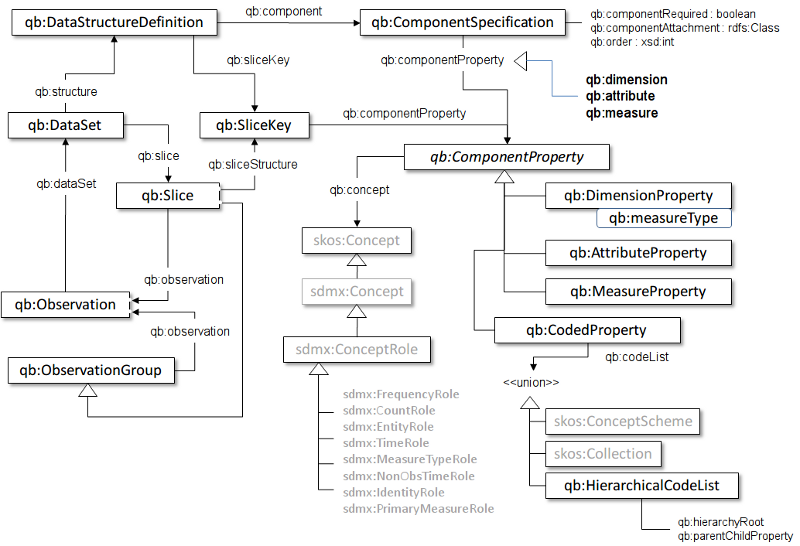
\includegraphics[width=\textwidth]{qb-fig1.png}
\caption{Outline des Data Cube Vokabulars}
\label{fig:my_label}
\end{figure}\\
So untergliedert sich ein DataCube in verschiedene DataSets, welche jeweils eine DataStructureDefinition besitzen, die die Komponenten des DataSets benennt. Diese Komponenten sind über die ComponentProperty entweder als Dimension, Attribut oder Measure (Messwert) definiert. Die ComponentPropertys besitzen ein direktes Mapping zu skos:Konzepten. Beschrieben wird der DataCube über Slices, also dimensionale Schnitte, welche Observations als Platzhalter für tatsächlich beobachtete Werte enthalten. Solche Observations müssen genau einem DataSet zugeordnet sein und für jede der MeasureProperties einen Wert im Rahmen des Definitionsbereiches auszeichnen.\\
Ein solcher DataCube kann in einem Triplestore gepflegt und über vernetzte Abfragen in Sparql können Sichten auf die darin enthaltene Statistik erzeugt werden (Betrachtung der Slices).
\subsection{DSSN / xodx}

Soziale Netzwerke stellen eine der aktuellen Schlüsselanwendungen des Web dar. Aufgrund der schieren Zahl der Benutzer und der geteilten Daten stehen Netzwerke wie Facebook mitunter zu Recht in der Kritik von Datenschützern. Dies und die Erforschung der Möglichkeiten des Semantic Web sowie Erschließung neuer Anwendungsfelder führte zur Entwicklung von xodx\cite{xodx_paper} am Lehrstuhl.\\
Es handelt sich dabei um eine Software für ein soziales Netzwerk, welches nach einem dezentralen, semantischen Paradigma erstellt wurde, kurz DSSN. Es nutzt für das Management seines dem Linked Data Prinzip folgenden Datenmodell die ebenfalls am Lehrstuhl entwickelten Semantic Web Frameworks Erfurt\footnote{Erfurt: \url{https://github.com/AKSW/Erfurt}} bzw. Saft\footnote{Saft: \url{https://safting.github.io/}} sowie Semantic Pingback\footnote{Semantic Pingback: \url{http://aksw.org/Projects/SemanticPingback.html}} als Kerntechnologie.\\
Die Funktionalität dieser Software sollte im Rahmen des Praktikums geprüft werden.

\subsubsection{Zend}

Bei Zend\footnote{Zend Framework: \url{http://framework.zend.com/}} handelt es sich um ein quelloffenes PHP Framework zur Erstellung komplexer Webanwendungen. Es verwendet dabei eine Strukturierung nach dem Designprinzip des MVC, also die Trennung von Model (dem Datenmodell der Webanwendung), Controllern (objektorientiert gekapselten Einheiten der ausführenden Programmlogik) und dem View (je nach Interpretation des Paradigmas mehr oder weniger funktionalen Nutzersicht der Anwendung).

\section{Vorarbeit}

Wie bereits in Kapitel 1 beschrieben, sollte die Arbeit auf der des Studententeams aus dem vergangenen Wintersemester aufsetzen und diese fortführen. Im letzten Jahr waren es 5, später 3 Studenten, welche an der Umsetzung einer Simulation für xodx arbeiteten. Die Arbeit umfasste drei Bereiche.
\begin{enumerate}
	\item{Entwicklung einer Test-Infrastruktur\\
	Es sollten virtuelle Container erstellt werden, auf welchen die xodx Soft-ware inklusive Virtuoso Backend läuft und welche untereinander auf getrennten Ports kommunizieren können. Zur Umsetzung dieser Aufgabe wurde Docker\footnote{Docker: \url{https://www.docker.com/}}gewählt. Dabei wurde geplant, dass jeweils eine Instanz von Docker auch genau eine Instanz der xodx Software, also einen Knoten im DSSN, umfasst und auf dieser Instanz nur ein Account registriert ist, welcher vom virtuellen Agenten bedient wird.}
	\item{Generierung von Testdaten\\
	Um eine möglichst realitätsgetreue Simulation zu erreichen, sollte ein Korpus aus Realdaten extrahiert und über Transformationen in eine mit Zeitstempel versehene Liste von Aktionen im sozialen Netzwerk generiert werden. Dazu wurde in Python eine App entwickelt, die über die Twitter-Api verschiedene, untereinander vernetzte Timelines extrahiert und nach XML parst.}
	\item{Planung einer Statistikkomponente\\
	Es sollte eine mögliche Umsetzung einer Statistikkomponente  recherchiert werden, um mit dieser die Software auf vorher festgelegte Fehlerklassen zu überprüfen. Als Fehlerklassen wurden Dateneffizienz, verlorene Nachrichten und Zugriffsgeschwindigkeit auf die eigene Zeitleiste festgestellt und es sollte mithilfe der Simulationssoftware ermöglicht werden, auf Unregelmäßigkeiten in diesen Gebieten zu prüfen. Die Speicherung der Daten dieser Erhebung sollte ebenfalls innerhalb des Paradigma des Semantic Web erfolgen und es wurde das DataCube Vokabular evaluiert sowie ein DataCube angelegt, der zur Speicherung der Daten verwendet werden soll. Es sollte das vom Lehrstuhl entwickelte Tool CubeViz\cite{cubeviz}\footnote{CubeViz Neuentwicklung: \url{https://github.com/AKSW/cubevizjs}} benutzt werden, um die Daten graphisch auszuwerten.}
\end{enumerate}
Mit dieser Arbeit war es möglich, dem eigentlichen Simulationsversuch näher zu kommen, auch wenn dieser aufgrund der geringen Teamgröße nicht umgesetzt werden konnte. Hier wurde im Wintersemester 2015/2016 erneut angesetzt mit dem Ziel, alle bereits vorhandenen Komponenten zu verbinden. Dazu wurde ein Replay Agent benötigt, welcher es ermöglicht, auf der laufenden Docker-Infrastruktur den vorhandenen Korpus ,,abzuspielen''.\\
 Zusätzlich dazu musste ein Statistik Controller als Verbindung zwischen der Live-Instanz eines Agenten und den im DataCube hinterlegten Beobachtungen entwickelt werden. Mit letzterer Aufgabe habe ich mich beschäftigt. Dabei ist mir aufgefallen, dass der im vergangenen Jahr erstellte DataCube bewusst von der aktuellsten Empfehlung des W3C abweicht, um besser mit CubeViz zu harmonieren. Mit der Neuentwicklung von CubeViz und anderen Möglichkeiten der Auswertung (siehe Kapitel 6) ist diese Anpassung nicht mehr notwendig und der DataCube konnte auf die aktuelle Version des Vokabulars geupdatet werden.

\section{Struktur des DataCube}

Der DataCube für die Speicherung und Auswertung der Messwerte umfasst 5 Datasets, also 5 Messgrößen. Diese sind in Tabelle 1 aufgeführt. Der Zusammenhang zwischen dieser Struktur, der Simulationsdurchführung und den notwendigen Berechnungen zur Evaluation der genannten Fehlerklassen soll in Kapitel 6 beschrieben werden.
\begin{table}[ht]
\centering
\label{table1}
\begin{tabular}{|l|l|}
\hline
Dataset & Beschreibung \\ \hline
\texttt{xo:dataset-xoFollowers}       & Anzahl der Follower für einen Agenten            	\\ \hline
\texttt{xo:dataset-xoOUT}        & Ausgehende Nachrichten         \\ \hline
\texttt{xo:dataset-xoIN}        & Eingegangene Nachrichten             						\\ \hline
\texttt{xo:dataset-xoTriples}        & Anzahl gespeicherter triple auf einem Knoten        	\\ \hline
\texttt{xo:dataset-xoAccess}        & Zugriffszeit auf eigene Zeitleiste             		\\ \hline
\end{tabular}
\caption{DataSets im DSSN DataCube}
\end{table}\\
Jedes dieser Datasets ist durch eine Data Structure Definition näher beschrieben. Hier werden die für die Umsetzung des Datasets benötigten Dimensionen angehängt. Sie sind in Tabelle 2 auf der Folgeseite aufgelistet. Zusätzlich nennt die Data Structure Definition auch die jeweilige Messgröße, welche im DSSN DataCube für jedes DataSet eindeutig gewählt wurde.
\begin{table}[t]
\centering
\label{table2}
\begin{tabular}{|l|l|}
\hline
Dimension & Beschreibung \\ \hline
\texttt{xo:refAgent}       & Identifikationsnummer des Agenten            			\\ \hline
\texttt{xo:refTime}        & Zeitpunkt der Messung, auch verwendet als Slice Key	\\ \hline
\end{tabular}
\caption{Dimensionen im DSSN DataCube}
\end{table}\\
Jede Messung, also jede Observation, benötigt einen eindeutigen Bezeichner und ist genau einem Dataset zugeordnet. Sie umfasst stets zusätzlich zu den zwei Dimensionen aus Tabelle 2 den Messwert in der Dimension der Messgröße des Datasets. Es gibt im Repository dazu ein kurzes Beispiel\footnote{\url{https://github.com/DSSN-Practical/DSSN_Statistics/blob/master/observations/exampleObservations.ttl}}. In diesem sind Observations zu zwei Agenten enthalten, die sich gegenseitig folgen und zu zwei Zeitpunkten Nachrichten versenden, wobei zwischen Messzeitpunkt 1 und 2 eine Nachricht nicht korrekt übertragen wird.

\section{Architektur des Statistik Controllers}
Der Statistik Controller ist in PHP 5 implementiert und folgt dem von Zend verwendeten Architekturmodell MVC. Er stellt einen zusätzlichen Controller dar, der über den Bootstrapping-Prozess von xodx zur Verfügung gestellt wird und dessen Messergebnis ohne xodx-Layout direkt über die URL bzw. mit einem http-request\footnote{\url{https:github.com/DSSN-Practical/DSSN\_Statistics/blob/master/doc/example-request.php}} abfragbar ist.\\
Der Statistik Controller ist nach dem Klassenkonzept von PHP in öffentliche (public) und klasseninterne (private) Funktionen strukturiert und arbeitet mit dem Model, an welches Sparql Queries gestellt werden, um die benötigten statistische Kennwerte zu ermitteln. Eine Zusammenfassung der ,,public'' Funktionen ist in Tabelle 3 gelistet. \newpage
Diese Funktionen sind als ,,Actions'' formuliert, werden also vom Zend Bootstrapper gefunden und mit entsprechenden Einstellungen über die Schnittstelle verfügbar\footnote{verfügbare Actions: Die readStoreAction diente ausschließlich der Verhaltensanalyse der Software in Bezug auf die abgespeicherten Daten. Sie sollte in einer laufenden Produktivversion der Software nicht mehr aktiv sein, da über sie via http-request der gesamte innere Speicher des Knotens auslesbar ist.} gemacht.\\
\begin{table}[ht]
\centering
\label{table3}
\begin{tabular}{|l|l|}
\hline
\texttt{public function} & Beschreibung \\ \hline
\texttt{getStatsAction}       & Ermitteln der Kennwerte und Formatierung in turtle 	\\ \hline
\texttt{readStoreAction}      & Auslesen des Triplestores und Ausgabe	\\ \hline
\end{tabular}
\caption{,,public'' Funktionen des Statistik Controllers}
\end{table}\\
Die ,,private'' Funktionen dienen zur Kapselung der einzelnen Anfragen an das Model beim Erstellen der Observations in den einzelnen Datasets. Durch diese Auslagerung von Funktionalität wird eine höhere Robustheit und des Codes erreicht und sie dient außerdem dazu, die Fehlersuche stark zu vereinfachen.

\section{Planung der Simulation, Auswertung}

In diesem Kapitel sollen die bisherige Versuchsplanung der Simulation sowie die bisher erstellten Möglichkeiten zur Auswertung des DataCube zusammengefasst werden.\\
Wie in Kapitel 3 teilweise beschrieben, ist geplant, auf einem leistungsfähigen Server zahlreiche Instanzen von Docker mit http-Schnittstellen untereinander zu initialisieren und so ein virtuelles Netzwerk aus Docker Containern aufzubauen. In diesen Containern läuft jeweils eine Instanz von xodx inklusive Virtuoso als xodx Knoten. Auf diesem Knoten ist jeweils nur ein Nutzer registriert, für den stellvertretend der virtuelle Agent in Form eines Replay-Programmes agiert.\\
Die auszuführenden Aktionen sind an Realdaten, genauer an einem Twitter Export im xml Format, orientiert. Diese sind mit normierten Zeitstempeln und Identifikatoren für Agenten versehenen, werden jeder Instanz zur Verfügung gestellt und von der Replay Struktur des Agenten in Form von http-requests ausgeführt. Es gibt eine einheitliche Systemzeit auf dem Server, welche das Fortschreiten der Simulation sichert.\\
Zu regelmäßigen Zeitpunkten wird diese Simulationszeit angehalten und es wird eine Statistik erstellt. Dies ist notwendig, um während der Messung selbige nicht durch Aktionen der Agenten zu verfälschen. Zur Durchführung der Messung ist ein spezieller Agent nötig, der eine Liste der Verbindungen zu jedem aktiven Agenten besitzt und von diesen rekursiv die Antworten des Statistik Controllers (Observations) sammelAuslastungst und speichert.\\
Dieser besondere Agent besitzt auch den Datensatz des DataCube, dem in der Auswertungsphase die Observations hinzugefügt werden. Die Auswertung soll in vier Schritten geschehen.
\begin{enumerate}
	\item{Transformation\\
	Sowohl der DataCube als auch die Observations sind in zur Erhöhung der Lesbarkeit in turtle serialisiert. Für Schritt 2 ist es jedoch notwendig, dass die Dateien in RDF/XML vorliegen. Diese Umwandlung ist relativ einfach mit einem Kommandozeilen Tool namens ,,Raptor''\footnote{Raptor: \url{http://librdf.org/raptor/}} durchführbar. Ein Beispielbefehl dafür ist in Abbildung 2 zu sehen.
	\begin{figure}[ht]
	\centering
	\texttt{\$ rapper -i turtle -o rdfxml observations/exampleObservations.ttl  > observations/exampleObservations.rdf}
	\caption{Beispielbefehl Raptor}
	\end{figure}
	}\\
	Diese Transformation hat zudem den Vorteil, dass eventuelle Fehler im RDF Graphen wie zum Beispiel falsch zusammengefügte Zeilen oder fehlende Präfixe frühzeitig erkannt und bereits in diesem Schritt behoben werden können.
	\item{Überprüfung auf Validität bzw. Evaluation\\
	Der nächste Schritt ist die Validitätsprüfung des DataCube. Dafür liegt ein ausführbares Java Archiv\footnote{\url{https://github.com/DSSN-Practical/DSSN_Statistics/blob/master/SparqlTester/bin/CubeValidator.jar}} im Repository, welches unter Verwendung des Apache Jena Frameworks das DataCube File sowie die Observations in den Arbeitsspeicher liest und darauf die Sparql queries ausführen kann, welche vom W3C zur Validierung eines DataCube zur Verfügung gestellt wurden. Diese liegen im Verzeichnis \texttt{/evaluation}. Das Archiv ist für die Verwendung auf der Kommandozeile auslegt und nimmt dementsprechend Parameter entgegen. Leider ist es mit Apache Jena nur möglich, RDF/XML serialisierte Dateien einzulesen (siehe Schritt 1). Ein Beispielbefehl ist in Abbildung 3 zu sehen.\\
	\begin{figure}[ht]
	\centering
	\texttt{\$ java -jar SparqlTester/bin/CubeValidator.jar datacubes/dssn\_cubeXML.rdf observations/exampleObservations.rdf evaluation/}
	\caption{Beispielbefehl DataCube Validierung/Evaluation}
	\end{figure}\\
	Die Ausgabe ist eine Liste aller bestandener oder nicht bestandener Tests. Sollte ein Test nicht bestanden werden, ist auch ein kurzer Kommentar und die fehlgeschlagene query zu sehen. Sollten zum Beispiel im Verlauf der Simulation der unwahrscheinliche Fall eintreten, dass zwei Observations den gleichen Bezeichner vom Zufallsgenerator zugewiesen bekommen, würde ein solcher Fehler an dieser Stelle herausgefiltert und könnte behoben werden.
	}
	\item{Überprüfung auf verlorene Nachrichten\\
	Dies ist die erste zu prüfende Klasse von Fehlern, welche während der Simulation auftreten können. Da in xodx die Versendung von Nachrichten auf Basis eines Abonnement eines anderen Nutzers geschieht und dieses Abonnement dezentral gespeichert wird, ist es für einen Nutzer von seinem eigenen Knoten aus nicht nachvollziehbar, an wie viele Rezipienten die Nachricht in seiner Zeitleiste versendet wurde. Diese Information lässt sich nur aus der Gesamtheit der Daten in der Statistik schließen. Hierfür wurde ebenfalls ein ausführbares Java Archiv geschrieben. Mit diesem ist es möglich, beliebige Sparql queries auf der Wissensbasis bestehend aus DataCube und Observations auszuführen. Einige für die Auswertung prädestinierte queries befinden sich im Unterordner \texttt{/queries}. In Abbildung 4 ist der Befehl für die Auswertung auf verlorene Nachrichten zu sehen.
	\begin{figure}[ht]
	\centering
	\texttt{\$ java -jar SparqlTester/bin/SelectTester.jar datacubes/dssn\_cubeXML.rdf observations/exampleObservations.rdf queries/checkLostMessages.sparql}
	\caption{Beispielbefehl Test auf verlorene Nachrichten}
	\end{figure}\\
	Dabei ist zu beachten, dass bei einem neuen Abonnement in xodx die gesamte Zeitleiste des Users ,,nachgezogen'' wird, weshalb alle versandten und empfangenen Nachrichten immer von Beginn der Simulation gezählt werden.
	}
	\item{Visualisierung: Dateneffizienz und Zugriffszeit\\
	Diese beiden Fehlerklassen eigenen sich besonders dafür, in einer Grafik wie zum Beispiel einem Graphenplot ausgewertet zu werden. Dafür kann der DataCube inklusive Observations zum Beispiel in CubeViz eingelesen werden und mit diesem Tool automatisch eine Visualisierung der Zeitverläufe der gespeicherten Triples und der eventuell ansteigenden Zugriffszeit erstellt werden. Leider war zum Zeitpunkt des Praktikums kein Release des neu entwickelten CubeViz verfügbar, um diesen Prozess zu testen.	
	}
\end{enumerate}

\section{Zusammenfassung}

Das Ziel des Praktikums war es, eine agentenbasierte Simulation als Belastungs- und funktionalem Test der xodx Software zu konzipieren, die dafür fehlenden Komponenten zu implementieren und die Simulation durchzuführen.\\
Dafür gab es eine umfangreiche Vorarbeit aus dem letzten Wintersemester, welche Docker Container zum Aufbau der Versuchsinfrastruktur, einen Korpus mit Live-Daten für die Simulation sowie ein Konzept und einen DataCube für die Auswertung bzw. statistische Überwachung des Versuchsablaufes beinhaltete.\\
Folglich bestanden die Aufgaben dieses Jahr darin, zum einen den Replay Agenten als Bindeglied zwischen der Docker/ xodx Instanz und dem Korpus und zum anderen einen Statistik Controller zum Messen und Sammeln der statistischen Kenngrößen zur Auswertung und Überwachung der Simulation zu implementieren.\\
Diese Aufgaben übernahmen ein Kommilitone und ich, wobei er leider ab der zweiten Hälfte des Semesters das Praktikum aus Zeitgründen abbrechen musste. Aus diesem Grund war es uns nicht möglich, die Aufgaben bis zur Durchführung der eigentlichen Simulation zu lösen.\\
Allerdings war die Umsetzung und der Test des Statistik Controllers auf einer lokalen Instanz von xodx mit einfachen Testdatensätzen erfolgreich und auch das Auswertungskonzept mit dem In-Memory Store von Apache Jena funktioniert und ist erweiterbar konzipiert.\\
Auch war es gut möglich, den DataCube vom letzten Jahr an die Ergebnisse der Analyse der xodx Software anzupassen sowie auf die neueste Version zu updaten und, ebenfalls via Apache Jena, einen einfachen Mechanismus zur Verifikation der Daten durch Evaluation des DataCube anhand der vom W3C vorgegebenen Constraints zu implementieren. \\
Zu diesen konzeptionellen Änderungen gehörten die Umsetzung der ,,Folgen''-Beziehung als einseitig gerichtetes Prädikat sowie die Umsetzung der xodx Funktionalität in der Auswertung der Simulation, dass beim Hinzufügen eines Freundes dessen gesamte Timeline ,,nachgezogen'' wird.\\
Mit dieser Struktur sollte es nun relativ einfach realisierbar sein, in einer weiteren Iteration der Testentwicklung für xodx eine agentenbasierte Simulation umzusetzen und den Praxistest der Software durchzuführen. Dafür fehlt noch der bereits angesprochene Replay Agent sowie ein spezieller Statistik Agent, der in den Pausenzeiten des Systems http-requests an alle registrierten Agenten stellt und die Antworten in z.B. einem File sammelt.\\
Es wäre auch denkbar, dass in den Pausenzeiten die aktivierten Agenten diese requests an sich selbst stellen und die Ergebnisse, welche mit einem Zeitstempel versehen sind, im Nachhinein eingesammelt und zusammengefügt werden.\\ 
Zusätzlich dazu müsste vom Lehrstuhl ein Server zur Verfügung gestellt werden, der die Last vieler parallel arbeitender Virtuoso Instanzen stemmen kann.

\newpage
\bibliographystyle{plain}
\bibliography{references.bib}
\end{document}
